\documentclass[DIV=1]{scrartcl}
%\documentclass[twocolumn, fontsize=8pt, DIV=1]{scrartcl}
\KOMAoptions{fontsize=20pt}
\usepackage[utf8]{inputenc}
\usepackage{natbib}
\usepackage{graphicx}
\usepackage{fancybox}
\usepackage{framed}
\usepackage{amsmath}
\usepackage{amssymb}
\usepackage{todonotes}
\usepackage[top=0.2cm, bottom=1.35cm, left=.2cm, right=.2cm]{geometry}
\usepackage[mark]{gitinfo2}

% Deutsche Anpassungen/Übersetzungen einbinden 
\usepackage[ngerman]{babel}

% Einzug der jeweils ersten Zeile verhindern
\setlength{\parindent}{0em}

% 4 on 1
\usepackage{pgfpages}
\pgfpagesuselayout{4 on 1}[a4paper,border shrink=5mm]

% Eigene Befehle für die Anordnung als näherungsweise Karteikarten
\newcommand{\frage}[3][10]{
    \newpage
    \ 
    \vspace{#1 em}
    \begin{framed}
        #2
    \end{framed}
    \newpage
    \begin{framed}
        #2
    \end{framed}
    \vspace{2 em}
}

%\renewcommand{\frage}[3][1]{
%    \vspace{#1 em}
%    \begin{framed}
%        #2
%    \end{framed}
%    \vspace{1 em}
%}

\title{GDF Fragen}
\subtitle{Sommersemester 2018}
\author{Nachos con queso \& GDF-Crew}
\date{}


\begin{document}

\maketitle \newpage
\ \newpage





%\section{Tensorrechnung}



\frage{Ko- bzw. kontravariante Basen}

Kovariante Basis unten, kontravariante Basis oben:
\[ \underline{g}_{i}\ \underline{g}^{j} = \delta_i^j = E \]

Vektor kann geschrieben werden:
\[ 
 \underline{v} = v^i \ \underline{g}_i = v_i \ \underline{g}^i 
\]

Die Länge von Vektoren und Winkeln zwischen Vektoren hängen nicht vom gewählten Basissystem ab (Invariante). Daher müssen bei schiefwinkligen Koordinatensystemen zur Berechnung des Skalarproduktes außer den Komponenten die zugehörigen Basisvektoren einbezogen werden.\\
\ \\
Mit $\underline{v} = v^i \ \underline{g}_i$ und $\underline{u} = u^j\ \underline{g}_j$:
\[
    \underline{v} \cdot \underline{u} = v^i \ \underline{g}_i \cdot u^j\ \underline{g}_j
    %= v^i\, u^j\ \underline{g}_i \cdot \underline{g}_j 
    = v^i\, u^j\, g_{ij}
    = v_i\, u_j\, g^{ij}
    = v_i\, u^j\, g^i_j
    = v_i\, u^j\, \delta^i_j
    = v_i\, u^j
\]
Kovarianter Metriktensor: \[g_{ij}\]
Kontravarianter Metriktensor: \[g^{ij}\]
Gemischter Metriktensor: \[\delta^i_j = g^i_j\]



\frage{Multiplikation, Überschiebung, Verjüngung}

Addition:
\[
    C_i = A_i + B_i
\]
Skalare Multiplikation:
\[
    B_i = a\, A_i
\]
Multiplikation:
\[
    C_{ik} = A_i\, B_k
\]
Einsteinsche Summenkonvention:
\[
    A^i\, B_i\ \hat{=}\ \sum_{i=1}^n A^i\, B_i
    \qquad\qquad\qquad
    A^i_i\ \hat{=}\ \sum_{i=1}^n A^i_i
\]
Überschiebung (bedeutet z.B. Skalarprodukt, Matrizenprodukt, $\dots$):
\[
    a = B_i\, C^i
    \qquad
    A_{ik} = B_i^j\, C_{jk}
    \qquad
    A_{ikl} = B_i^j\, C_{jkl}
\]
Verjüngung (Stufe des Tensors wird um 2 herabgesetzt):
\[
    A^i_i = A^1_1 + \dots + A^n_n = a \qquad \text{Spur einer Matrix}
\]
\[
    A^i_{ijk} = A^1_{1jk} + \dots + A^n_{njk} = B_{jk}
\]



\frage{Transformationsverhalten Tensoren}

\todo[inline]{Wer formuliert was hübsches?\ \ \ \ \ (-:}



\frage{Beispiele für Tensoren}

Tensor 0. Stufe: Skalar\\
Tensor 1. Stufe: Vektor\\
Tensor 2. Stufe: Matrix\\
Tensor 3. Stufe: \glqq räumliche Matrix\grqq
\[
    a \qquad A_i,\ A^i \qquad A_{ij},\ A_{i}^j,\ A^{ij} \qquad A_{ijk} \qquad \dots
\]








%\section{Kurventheorie}



\frage{Wie werden Kurven parametrisiert?}

Vektorwertige Funktion:
\[
\underline{X} : \  I \in \mathbb{R} \to \mathbb{R}^3, \qquad 
\underline{X}(t) =
 \left(
 \begin{array}{c}
 x_1(t)\\
 x_2(t)\\
 x_3(t)
 \end{array}
\right) 
\]



\frage{Was zeichnet Bogenlängenparametrisierung aus?}

\[
|\underline{X}'| = 1
\]
Der Parameter gibt gleichzeitig die Bogenlänge von $0$ bis $s$ an.



\frage{Was ist das begleitende Dreibein einer Kurve? Aus welchen Vektoren besteht es?}

Bei Bogelängenparametrisierung: lokales, orthogonales Koordinatensystem.\\
\\
Tangentenvektor:
\[
    \underline{v}_1 = \underline{X}'
\]
Hauptnormalenvektor:
\[
    \underline{v}_2 = \frac{\underline{X}''}{||\underline{X}''||}
\]
Binormalenvektor:
\[
    \underline{v}_3 = \underline{v}_1 \times \underline{v}_2
\]
$\underline{v}_2$ zeigt in die Richtung des Krümmungskreismittelpunktes.



\frage{Was bedeutet Bogenlänge und wie wird sie berechnet?}

Länge eines Stückchens Kurve.
\[
    s(t) = \int_{t_0}^t ||\underline{\dot{X}}(\tau)||\, d\tau
\]




\frage{Was bedeutet Krümmung und wie wird sie berechnet?}

Die Krümmung in einem Kurvenpunkt entspricht der Krümmung des Schmiegkreises.
Sie ist das Maß, wie stark die Kurve vom geradlinigen Verlauf abweicht.\\
\\
Bei Bogenlängenparametrisierung:
\[
    \kappa(s) = ||\underline{\ddot{X}}(s)||
\]



\frage{Was bedeutet Torsion und wie wird sie berechnet?}

Die Torsion beschreibt, wie stark sich die Kurve aus der Schmiegebene herauswindet.
\[
    \tau(t) = \frac{\det(\underline{\dot{X}}(t), \underline{\ddot{X}}(t), \underline{\dddot{X}}(t))}{||\underline{\dot{X}}(t) \times \underline{\ddot{X}}(t)||^2}
\]



\frage{Was ist an Bogenlänge, Krümmung und Torsion besonders?}

\begin{itemize}
    \item sind geometrische Invarianten
    \item hängen nicht von der mathematischen Beschreibung der Kurve ab
    \item Kurve ist bis auf Bewegungen im Raum durch diese 3 Größen eindeutig bestimmt
\end{itemize}



\frage{Wann ist eine Kurve eben?}

Wenn die Torsion $0$ ist.



\frage{Welchen Zusammenhang beschreiben die Frenet-Formeln und welche Größen kommen darin vor?}

Es sind Differentialgleichungen, die die Änderung des Dreibeins angeben, also den Zusammenhang zwischen den Vektoren des Frenet-Dreibeins und deren Ableitungen.
\begin{itemize}
    \item Die Vektoren des Dreibeins
    \item Die Ableitungen der Vektoren des Dreibeins
    \item Krümmung $\kappa$
    \item Torsion $\tau$
\end{itemize}



\frage{Wie heißen die Ebenen, die von den Vektoren des begleitenden Dreibeins aufgespannt werden?}

Schmiegebene:
\[
    \underline{v}_1,\ \underline{v}_2
\]
Rektifizierende Ebene:
\[
    \underline{v}_1,\ \underline{v}_3
\]
Normalebene:
\[
    \underline{v}_2,\ \underline{v}_3
\]



\frage{Wohin zeigt der Hauptnormalenvektor einer Kurve?}

Der Hauptnormalenvektor einer Kurve zeigt in Richtung Krüm\-mungs\-krei\-smit\-tel\-punkt.











%\section{Flächentheorie}



\frage{Wie werden Flächen parametrisiert?}

Vektorwertige Funktion:
\[
\underline{X}: \quad G \in \mathbb{R}^2 \to \mathbb{R}^3, \qquad 
\underline{X}(u^1, u^2) =
 \left(
 \begin{array}{c}
 x_1(u^1, u^2)\\
 x_2(u^1, u^2)\\
 x_3(u^1, u^2)
 \end{array}
\right) 
\]



\frage{Wann heißt eine Punktmenge $\underline{X}(u^1, u^2)$ reguläres Flächenstück?}

\begin{itemize}
    \item $\underline{X}$ injektiv (keine Selbstüberschneidungen
    \item $\underline{X}_1 \times \underline{X}_2 \neq \underline{0}\ \ \ \forall\ (u^1, u^2) \in G$
    \item $\underline{X} \in C^3$
\end{itemize}



\frage{Wann heißt eine Parametertransformation bei Flächen zulässig?}

\begin{itemize}
    \item Funktionaldeterminante $\neq 0$
    \item $u^1, u^2 \in C^3$
\end{itemize}



\frage{Wie berechnet man die Tangentialebene und was bedeutet sie?}

Analog zur Tangente bei Kurven berührt die Ebene die gegebene Fläche tangential. Voraussetzung ist, dass eine Flächennormale existiert.
\[
    T(\mu_1, \mu_2) = \underline{X}(u^1_0, u^2_0) + \mu_1 \underline{X}_1(u^1_0, u^2_0) + \mu_2 \underline{X}_2(u^1_0, u^2_0),
    \qquad \mu_i \in \mathbb{R}
\]


\frage{Wie berechnet man die Flächennormale und was bedeutet sie?}

Die Flächennormale steht orthogonal auf der Tangentialebene. In regulären Flächenstücken ist $\underline{N} \neq 0$.
\[
    \underline{N}(u^1_0, u^2_0) = \frac{\underline{X}_1(u^1_0, u^2_0) \times \underline{X}_2(u^1_0, u^2_0)}{||\underline{X}_1(u^1_0, u^2_0) \times \underline{X}_2(u^1_0, u^2_0)||}
    \qquad \qquad
    \underline{N} = \frac{\underline{X}_1 \times \underline{X}_2}{||\underline{X}_1 \times \underline{X}_2||}
\]


\frage{Was bedeutet orientierbar?}

Die Richtungsänderung der Normalen von Punkt zu Nachbarpunkt ist stetig.\\
\\
Gegenbeispiele: Möbiusband, Kleinsche Flasche



\frage{Wie werden die 1. Fundamentalgrößen berechnet?}

\[
    g_{ik} =
        \left(
            \begin{array}{rr}
                g_{11} & g_{12} \\
                g_{21} & g_{22}
            \end{array}
        \right) =
        \left(
            \begin{array}{rr}
                \langle \underline{X}_1, \underline{X}_1 \rangle & \langle \underline{X}_1, \underline{X}_2 \rangle \\
                \langle \underline{X}_2, \underline{X}_1 \rangle & \langle \underline{X}_2, \underline{X}_2 \rangle
            \end{array}
        \right)
        , \qquad \text{mit}\ g_{12} = g_{21}
\]



\frage{Was kann man mit den 1. Fundamentalgrößen ausrechnen?}

\begin{itemize}
    \item Längen von und Winkel zwischen Flächenkurven
    \item Flächeninhalt
    \item Länge der Kurve auf einer gegebenen Fläche
    \item Gauß-Krümmung: $K = \kappa_1 \cdot \kappa_2$
    \item Christoffel-Symbole 2. Art
\end{itemize}



\frage{Wann ist ein Parametersystem orthogonal?}

Wenn die partiellen Ableitungen orthogonal zueinander sind:
\[
    g_{12} = g_{21} = 0
\]



\frage{Wie werden die 2. Fundamentalgrößen berechnet?}

Skalarprodukte aller 2. partiellen Ableitungen mit $\underline{N}$:
\[
    L_{ik} =
        \left(
            \begin{array}{rr}
                \langle \underline{X}_{11}, \underline{N} \rangle & \langle \underline{X}_{12}, \underline{N} \rangle \\
                \langle \underline{X}_{21}, \underline{N} \rangle & \langle \underline{X}_{22}, \underline{N} \rangle
            \end{array}
        \right)
\]



\frage{Was ist das begleitende Dreibein der Fläche?}

Tangentenvektor in $u^1$-Richtung:
\[
    \underline{X}_1
\]
Tangentenvektor in $u^2$-Richtung:
\[
    \underline{X}_2
\]
Normalenvektor:
\[
    \underline{N}
\]
\\
\\
Im Skript:
\[
\underline{X}' \qquad \underline{N} \qquad \underline{S}
\]
mit $\underline{X}' = \underline{X}_i \, {u^{i}}'$ und  $\underline{S} = \underline{X}' \times \underline{N}$



\frage{Was ist die Normalkrümmung?}

Die Normalkrümmung einer Flächenkurve in einem Flächenpunkt $\underline{P}$ ist betragsmäßig gleich der Krümmung der sie in $\underline{P}$ berührenden ebenen Normalschnittes. \textbf{Achtung:} Der Normalschnitt benötigt eine Richtung!
\[
    \kappa_n = \frac{II}{I}
\]
Der Normalschnitt wird von dem Tangentenvektor und dem Normalenvektor aufgespannt. Jedoch fällt der Normalenvektor mit dem Hauptnormalenvektor zusammen, sodass die Richtung nicht eindeutig bestimmt ist.\\
\\
Die Richtung ist in den Fundamentalformen mit drin ($du^i, du^k$).


\frage{Was ist die geodätische Krümmung?}

Krümmung der Flächenkurve kann in zwei Anteile zerlegt werden: In Richtung der Flächennormalen (Normalkrümmung) und in Richtung des \glqq Seitenvektors\grqq\ $\underline{S} = \underline{N} \times \underline{X}'$ (geodätische Krümmung). \textbf{Achtung:} Für die geodätische Krümmung benötigen wir auch eine Richtung ($\underline{X}'$ ist auf eine Flächenkurve bezogen)!\\
\\
Die geodätische Krümmung gibt also an, wie ich \textbf{in} der Fläche gekrümmt laufe (innere Krümmung/Geometrie).\\
\\
Kürzeste Wege von einem Flächenpunkt zu einem anderen zeichnen sich so aus, dass die geodätische Krümmung $0$ ist.



\frage{Haben alle Flächenkurven mit gleicher Tangente in einem gemeinsamen Punkt auch gleiche Normalkrümmung?}

Eine Einschätzung:\\
\\
Ja, weil:\\
Die Normalkrümmung ist die Krümmung der Kurve, die durch Schnitt der Fläche mit einer Normalebene entsteht. Da beim Normalschnitt als einzige weitere Information eine Richtung auf der Fläche benötigt wird, und diese durch die Tangente gegeben ist, haben also auch alle Flächenkurven mit gleicher Tangente in einem gemeinsamen Punkt auch die gleiche Normalkrümmung.



\frage{Was ist und wie entsteht ein Normalschnitt?}

Beim Normalschnitt ist der Normalenvektor der Fläche linear abhängig mit dem Hauptnormalenvektor der Flächenkurve. Es gilt:
\[
    \underline{N} = \pm \underline{v}_2
\]



\frage{Wie hängt die Normalkrümmung mit der 1. und, 2. Fundamentalform zusammen?}

\vspace{-1em}
\[
    \kappa_n = \frac{II}{I}
\]



\frage{Was ist die Meusnier-Kugel?}

\begin{enumerate}
    \item Alle Schiefschnitte bilden (Schnittebenen aufgespannt durch: \\Einen Richtungsvektor und alle dazu orthogonalen Vektoren)
    \item Es entstehen Krümmungskreise
    \item Mit Krümmungskreisen ist die Meusier-Kugel vollständig definiert
\end{enumerate}
Der Krümmungskreis des Normalschnittes ist Großkreis der Meusnier-Kugel.



\frage{Was sind Hauptkrümmungen, Hauptkrümmungsrichtungen?}

Die Hauptkrümmungen $H$ sind die Extremwerte der Normalkrümmung.\\
\\
Hauptkrümmungsrichtung: zugehörige Tangentialrichtung.
\[
    \kappa_{1,2} = H \pm \sqrt{H^2 - K}
\]
Die Hauptkrümmungsrichtungen sind immer orthogonal zueinenander (ausgenommen z.B. Nabelpunkte, dort sind alle Richtungen Hauptkrümmungsrichtungen).\\
\\
Kugel: In jedem Punkt $\kappa_1 = \kappa_2$\\
Torsen: $\kappa_1 = 0,\ \kappa_2 > 0$\\




\frage{Wie berechnet man die Gaußsche Krümmung und mittlere Krümmung?}

Gaußsche Krümmung:
\[
    K = \kappa_1 \cdot \kappa_2
\]
Mittlere Krümmung:
\[
    H = \frac{\kappa_1 + \kappa_2}{2}
\]



\frage{Charakterisierung der Flächenpunkte: Elliptisch, hyperbolisch, parabolisch}

Elliptischer Flächenpunkt, z.B. Kugel:
\[
    K = \kappa_1 \cdot \kappa_2 > 0
\]
Hyperbolischer Flächenpunkt, z.B. Sattelfläche:
\[
    K = \kappa_1 \cdot \kappa_2 < 0
\]
Parabolischer Flächenpunkt (mind. eine Hauptkrümmung ist $0$), z.B. Zylinder:
\[
    K = \kappa_1 \cdot \kappa_2 = 0
\]
\\
\\
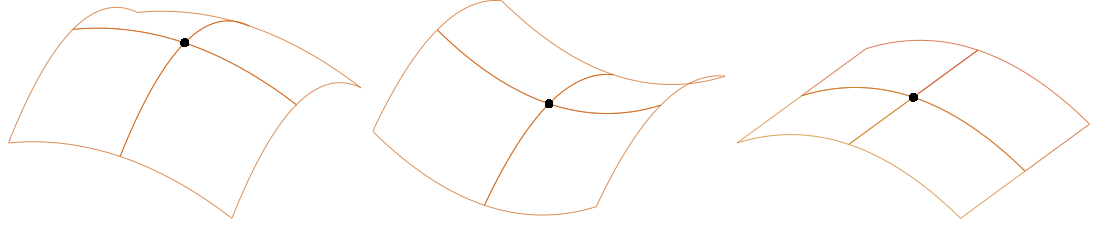
\includegraphics[scale=0.525]{elliptisch_hyperbolisch_parabolisch.png}



\frage{Was ist die Dupinsche Indikatrix?}

So wie ich es verstanden habe:\\
Wir nehmen die Tangentialebene und schieben sie infitessimal in Richtung und entgegen der Richtung der Normalen. Diese Ebenen schneiden wir dann mit der Fläche. Dadurch erhalten wir Informationen über die Krümmung in Form der Gleichung der Dupinschen Indikatrix.\\
\\
Hier die Beschreibung aus dem Skript:\\
Die zu einer beliebigen Richtung gehörende Normalkrümmung lässt sich durch die Hauptkrümmungen ausdrücken:
\textit{Zu einem Flächenpunkt, der weder Nabel- noch Flachpunkt ist, gilt für die Normalkrümmung $\kappa_n$ einer Flächenkurve, deren Tangente einen Winkel zur ersten Hauptkrümmungsrichtung hat:}
\[
    \kappa_n = \kappa_1\, \cos^2 \varphi + \kappa_2\, \sin^2 \varphi
\]
Mit $z_1\ \overset{\text{vermutlich}}{=}\ \frac{\cos\varphi}{\sqrt{\kappa_n}}$ und $z_2\ \overset{\text{vermutlich}}{=}\ \frac{\sin\varphi}{\sqrt{\kappa_n}}$ erhalten wir die Gleichung der Dupinschen Indikatrix:
\[
    \kappa_1\, z_1^2 + \kappa_2\, z_2^2 = \pm 1
\]


\frage{Was sind Krümmungslinien?}

Eine Krümmungslinie ist eine Flächenkurve, deren Tangente in jedem Punkt in eine der beiden Hauptkrümmungsrichtungen zeigt.\\
\\
Auf einem regulären Flächenstück sind die Parameterlinien $u^1 = const$ und $u^2 = const$ genau dann Krümmungslinien, wenn:
\[
    g_{12} = L_{12} = 0
\]
Beispiele:\\
\begin{itemize}
    \item Die auf einem Kreiszylinder liegenden Kreise und Geraden
    \item Die auf einem einschaligen Rotationshyperboloiden liegenden Kreise und dazu senkrechten Hyperbeln
    \item Kreise auf dem Dupinschen Zykloid
\end{itemize}



\frage{Wann sind die Parameterlinien Krümmungslinien (zeigen also in Hauptkrümmungsrichtungen)?}

Wenn:
\[
    g_{12} = L_{12} = 0
\]
\\
Bei Rotationsflächen sind die Parameterlinien immer Krümmungslinien (Meridiane und Breitenkreise).\\



\frage{ Was ist ein Flachpunkt?}

Hauptkrümmungen sind $0\ \Rightarrow$ alle Richtungen sind Haupt\-krüm\-mungs\-rich\-tung\-en, z.B. bei Ebene.
\[
    \kappa_1 = \kappa_2 = 0
\]



\frage{Was ist ein Nabelpunkt?}

Alle Richtungen sind Hauptkrümmungsrichtungen.
\[
    \kappa_1 = \kappa_2
\]



\frage{Welche Fläche hat nur elliptische Flächenpunkte?}

Die Oberfläche der Kugel besteht ausschließlich aus elliptischen Flächen\-punkten.



\frage{Wie lautet die 1. Fundamentalform?}

\[
    I: \ ds^2 = g_{ik}\, du^i\, du^k
\]



\frage{Was sind Asymptotenlinien?}

Richtungen, in denen die Normalkrümmung $0$ ist. Gibt es nur bei hyperbolischen ($K<0$) und elliptischen ($K>0$) Flächenpunkten.
\[
    \kappa_n = 0
\]
In hyperbolischen Flächenpunkten existieren stets zwei reelle Scharen von Asymptotenlinien, in parabolischen Flächenpunkten eine reelle Schar.\\
\\
Auf einem Rotationshyperboloid sind die beiden erzeugenden Geradenscharen Asymptotenlinien\\
\\
Aus Wikipedia:\\
Jede Erzeugende einer Regelfläche ist eine Asymptotenlinie der Regelfläche.




\frage{Wie werden Asymptotenlinien berechnet?}

\[
    L_{ik}\,\dot{u}^i\,\dot{u}^k = 0 \qquad \text{(DGL)}
\]



\frage{Was ist die Normalkrümmung einer Asymptotenlinie?}

\[
    \kappa_n = 0
\]



\frage{Wann sind Parameterlinien Asymptotenlinien?}

Parameterlinien sind Asymptotenlinien $\Leftrightarrow L_{11} = L_{22} = 0$.



\frage{Wie bekommt man geodätische Linien, kürzeste Wege auf Flächen?}
Durch die Ableitungsgleichungen von Gauß.
\[
    \kappa_g = 0 
    \qquad\qquad\qquad\qquad
    \kappa_g  = \underline{X}'' \cdot \underline{S} = \det(\underline{X}', \underline{X}'', \underline{S})
\]
\\
Dabei ist $\kappa_g$ der Anteil von $\kappa$ in der Tangentialebene und nur von der 1. Fundamentalform abhängig.\\
$\kappa_g$ ist Größe der inneren Geometrie der Fläche.\\
$\kappa_g$ gibt an, wie eine Kurve innerhalb der Fläche gekrümmt ist.



\frage{$ds$, was ist das?}

Ein infitessimal kleines Kurvenstück.



\frage{Was ist der Hyperboloid für ein Flächentyp?}

Windschiefe Regelfläche, die Tangentenfläche entlang der Erzeugenden ändert sich.
\\
\begin{center}
    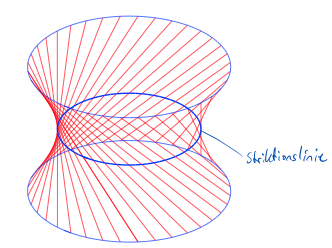
\includegraphics[scale=1]{hyperboloid.png}
\end{center}



\frage{Was ist der Kegel für ein Flächentyp? Gib mal ein $\kappa_1$ und ein $\kappa_2$ für einen Kegel an.}

Regelfläche, genauer: Torse. Eine Hauptkrümmung ist $0$.



\frage{Was ist der Zylinder für ein Flächentyp? Gib mal ein $\kappa_1$ und ein $\kappa_2$ für einen Zylinder an.}

Regelfläche, genauer: Torse. Eine Hauptkrümmung ist $0$.
\\
\begin{center}
    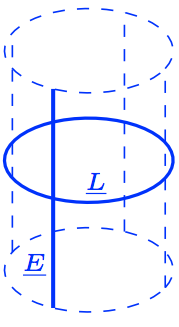
\includegraphics[scale=1]{zylinder.png}
\end{center}











%\section{Ableitungsgleichungen}



\frage{Gibt es immer zu zulässig vorgegebenen $g_ik$ und $L_ik$ ein Flächenstück?}

Nicht ohne Weiteres. Man benötigt weitere Verträglichkeitsbedingungen, die Integrabilitätsbedingungen von Gauß und Mainardi-Codazzi.



\frage{Welche Größen setzen die Ableitungsgleichungen von Gauß in Beziehung?}

Die Ableitungsgleichungen von Gauß setzen
\begin{itemize}
    \item die ersten partiellen Ableitungen
    \item die zweiten partiellen Ableitungen 
    \item den Normalenvektor
\end{itemize}
eines Flächenstücks in Beziehung.
\[
    \underline{X}_{ik} = \Gamma_{ik}^r \, \underline{X}_r + L_{ik} \, \underline{N}
\]



\frage{Aus welchen Größen lassen sich die Christoffel-Symbole berechnen?}

Aus den 1. Fundamentalgrößen ($g_{ik}$) und deren Ableitungen.



\frage{Welche Größen setzen die Ableitungsgleichungen von Weingarten in Beziehung?}

Ergebnis: Ableitung des Normalenvektors\\
Benötigt:
\begin{itemize}
    \item 1. Fundamentalgrößen
    \item 2. Fundamentalgrößen
    \item Partielle Ableitung des Flächenstücks
\end{itemize}
\[
    \underline{N}_k = - L_{jk} \, g^{jr} \, \underline{X}_r
\]



\frage{Verträglichkeitsbedingungen von Gauß und Mainardi-Codazzi: Wenn sie erfüllt sind, was hat das zur Folge?}

Satz 3.6.1:\\
Erfüllen die 1. und 2. Fundamentalgrößen die partiellen Differentialgleichungen von Gauß und Mainardi-Codazzi (Integrabilitätsbedingungen), dann gibt es ein eindeutiges, reguläres Flächenstück (bis auf Bewegungen im Raum).\\
\\
Die 1. und 2. Fundamentalgrößen sind über die Integrabilitätsbedingungen gekoppelt. Durch diese wird die Vertauschbarkeit höherer partieller Ableitungen gesichert.



\frage{Welche Größen stecken im Riemannschen Krümmungstensor?}

Zusammenhang zwischen 1. und 2. Fundamentalgrößen:
\[
    R_{ikl}^l = L_{ik} \, L_j^l - L_{ij} \, L_k^l
\]



\frage{Was sagt uns das Theorema Egregium von Gauß?}

\textit{Die Gaußsche Krümmung $K$ ist eine Größe der inneren Flächen\-geometrie. Sie lässt sich allein aus den $g_{ik}$ und Ableitungen der $g_{ik}$ bestimmen. Es gilt:}
\[
    K = \frac{g_{1k}}{g} \, R_{212}^k
\]
$R_{ikl}^l$ ist der Riemannsche Krümmungstensor.











%\section{Spezielle Flächen: Regelflächen}



\frage{Wie lautet die Parametrisierung einer Regelfläche?}

\[
    \underline{X}(u^1, u^2) = \underline{L}(u^1) + u^2\, \underline{E}(u^1)
    \quad \text{mit} \quad ||\underline{E}(u^1)|| = 1
\]



\frage{Was ist eine Leitkurve, was sind Erzeugende?}

Erzeugende:\\
Geraden (bei windschiefen Regelflächen sind es windschiefe Geraden)\\
\\
Leitkurve:\\
Hier werden die Erzeugenden entlang geschoben.




\frage{Wodurch unterscheiden sich Torsen von windschiefen Regelflächen?}

Torse:\\
Regelfläche, bei der die Tangentialebene in einem beliebigen Flächenpunkt zugleich Tangentialebene in allen anderen Punkten derselben Erzeugenden ist. Torsen haben also keinen Drall ($\frac{d\varphi}{dl}$, Winkeländerung von zwei benachbarten Erzeugenden).\\
Eine Fläche ist genau dann Torse, wenn $\det(\underline{L}_1, \underline{E}, \underline{E}_1) = 0$ (Torsenbedingung).\\
\textbf{Torsen sind} entweder \textbf{Zylinder, Kegel oder Tangentenflächen}.\\
\\
Windschiefe Regelfläche:\\
Benachbarte Erzeugende sind stets windschief.




\frage{Welche Eigenschaften haben Striktionspunkte, Striktionslinie?}

Die Striktionslinie ist die Menge aller Striktionspunkte.\\
\\
Striktionspunkt: Die Grenzlage der Lotfußpunkte des Gemeinlots zweier benachbarter Erzeugenden.



\frage{Aus welchen Vektoren besteht das begleitende Dreibein einer Regelfläche?}

Das begleitende Dreibein einer Regelfläche besteht aus:\\
\\
Erzeugende:
\[
    \underline{E}
\]
Zentralnormale:
\[
    \underline{Z}_n = \frac{\underline{E}_1}{||\underline{E}_1||}
\]
Zentraltangente:
\[
    \underline{Z}_T = \underline{E} \times \underline{Z}_N
\]
In anderen Worten:\\
Aus der Erzeugenden, der Ableitung und dem Kreuzprodukt der beiden.




%\newpage
%\listoftodos


\end{document}
